\subsection{Retained admission ledger and pre-decision margins}\label{app:latest-admissions}

% Figures 14 and 15 (cited in Appendices D.2 and D.3) are defined here, at the
% start of Appendix D, so both full-width figures head the next page; defined
% after their sections, they slipped a page whenever the text above grew.
\begin{figure*}[t]
  \setlength{\abovecaptionskip}{4pt}
  \centering
  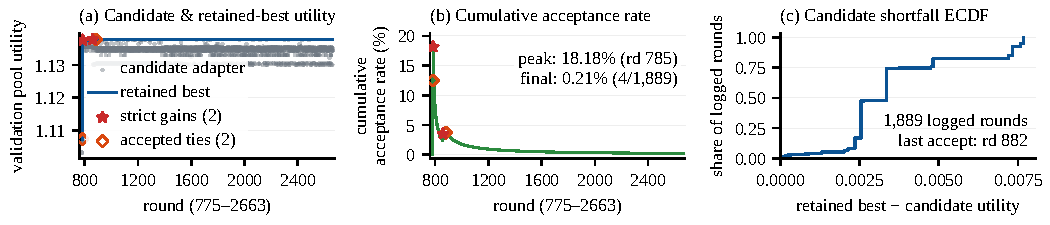
\includegraphics[width=\linewidth,height=1.50in,keepaspectratio]{figures/fig_fw_acceptance_over_rounds.pdf}
  \caption{\textbf{Cumulative adapter acceptance falls to 0.21\% across rounds 775--2663.}
  All three panels use the same \num{1889} consecutive admission evaluations (\cref{tab:admission-ledger}).
  (a) Candidate validation utility (logged scalar score; grey) and post-decision recorded best (blue), with stars at
  strict gains (rounds 785 and 859) and hollow diamonds at accepted ties (rounds 782 and 882).
  (b) Cumulative accepted share of elapsed rounds (\%), peaking at 18.18\% at round 785 and
  declining across \num{1781} subsequent rejected rounds to 0.21\% ($4/\num{1889}$).
  (c) Empirical cumulative distribution (fraction of evaluations) of recorded-best minus candidate validation utility;
  zero marks the four accepted adapter evaluations. Scope: \cref{sec:method-status}.}
  \label{fig:fw-validation}
  \label{fig:fw-acceptance-over-rounds}
  \label{fig:fw-admission-shortfall}
\end{figure*}
\begin{figure*}[!t]
  \setlength{\abovecaptionskip}{4pt}
  \centering
  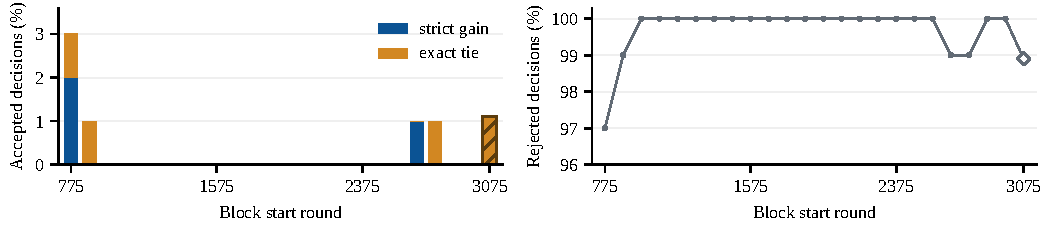
\includegraphics[width=\linewidth,height=1.55in,keepaspectratio]{figures/fig_fw_admission_block_rates.pdf}
  \caption{\textbf{Nineteen of 24 observed-round blocks record zero adapter admissions.}
  All \num{2391} complete journal decisions in rounds 775--3165, captured at 20:17 UTC
  on 1 November 2026. Blocks contain 100 consecutive observed rounds; the final
  3075--3165 block contains 91. Left: accepted strict gains (blue) and exact ties
  (orange), stacked percentages. Right: rejected decisions (\%; axis starts
  at 96\%). Each denominator is that block's observed rounds; hatching and a
  diamond mark the partial block. Totals: three strict gains, four ties and
  \num{2384} rejections. These adaptive adapter decisions are distinct from
  program-incumbent events and independent first-proposal \mbox{game-day performance. Scope: \cref{sec:method-status}.}}
  \label{fig:fw-candidate-retained-trace}
\end{figure*}

\begin{table}[!htbp]
  \caption{\textbf{The canonical admission ledger records every complete row in the prefix.}
  Strict gains and ties use unrounded candidate minus prior-best
  utility, without outcome selection. Scope: \cref{sec:method-status}.}
  \label{tab:admission-ledger}
  \centering\footnotesize\setlength{\tabcolsep}{4pt}\renewcommand{\arraystretch}{0.92}\sisetup{group-digits=integer}% full-precision logged values: roman digits and a true minus
  \begin{tabularx}{\linewidth}{@{}>{\raggedright\arraybackslash}Xl@{}}
    \toprule
    Quantity & Recorded value \\
    \midrule
    Capture cutoff (UTC) & 2026-11-02 23:00 \\
    Complete rounds & 775--3950 (\num{3176} records) \\
    Admissions / rejections & 8 / \num{3168} \\
    Strict-gain rounds & 785, 859, 2750, 3175 \\
    Exact-tie rounds & 782, 882, 2795, 3100 \\
    Final retained utility & \num{1.1389572403748425} \\
    Recorded best-round identity & 3175 \\
    New rows since prior capture & 753 (0 admitted) \\
    Rejected margins in $[-10^{-4},0)$ & 26 \\
    Rejected margins in $[-10^{-3},-10^{-4})$ & 51 \\
    Rejected margins below $-10^{-3}$ & \num{3091} \\
    Closest rejected margin & \num{-0.0000433838086485} (round 803) \\
    Median rejected margin & \num{-0.0033601045139468} \\
    \bottomrule
  \end{tabularx}
\end{table}

\Cref{tab:admission-ledger} collects the chronology, exact counts and
margin summaries for one capture. The pre-decision margin is
$\Delta_r=u_{\mathrm{cand},r}-u_{\mathrm{prev},r}$;
the default rule accepts $\Delta_r\geq0$.

\Cref{fig:fw-admission-margins} summarizes complete trailing 50-round
windows and cumulative near-tie rejections from that same record.
